\documentclass[a4paper,14pt]{extarticle}
\usepackage[a4paper,top=2.0cm, bottom=1.5cm, left=2cm, right=1.5cm]{geometry}
\usepackage[T2A]{fontenc}			
\usepackage[utf8]{inputenc}		
\usepackage[english,russian]{babel}	
\usepackage{amsmath,amsfonts,amssymb,amsthm,mathtools} 
\usepackage{wasysym}
\usepackage{graphicx}
\usepackage{wrapfig}
\usepackage{amsmath}
\usepackage{ mathrsfs }
\usepackage{caption}
\usepackage{subcaption}
\usepackage{multirow}
\DeclareMathOperator*{\argmax}{argmax}
\DeclareMathOperator*{\argmin}{argmin}
\DeclareGraphicsExtensions{.pdf, .png, .jpg}
\graphicspath{{}}
\linespread{1.5}



\begin{document}
	\vspace*{\fill}
	\begin{abstract}	
	 	Исследуются задачи связанные с образами (составленными из элементов одежды), в частности задача дополнения образа. Рассматриваются препятствия к точному решению задачи и его аппроксимациям. Решается задача нахождения эффективного алгоритма построения дополнения. Обосновываются несколько методов аппроксимации точного решения, в частности, наиболее успешно себя показавшая генерация скрытых представлений для элементов дополнения. Производится сравнение рассматриваемых подходов. Теоретически поясняется экспериментально показанное преимущество генерации скрытых представлений над прочими рассмотренными подходами.
	\end{abstract}
	\vspace*{\fill}
\newpage
	
	\section{Введение}
		В последние годы, методы машинного обучения позволяют добиваться успехов в задачах рекомендации, однако задачи требующие подбора группы объектов совместимых между собой, все еще представляют серьезную проблему. Основным препятствием к решению в таких случаях является неизвестный характер зависимости между объектами в группах. В работе исследуется необходимость и способы построения аппроксимации этой зависимости для прикладной задачи рекомендации наборов одежды называемых <<образами>>. 
		В частности, в отличие от ранее представленных работ \cite{https://doi.org/10.48550/arXiv.1908.11754} \cite{https://doi.org/10.48550/arXiv.2005.12566}  \cite{https://doi.org/10.48550/arXiv.2204.04812}, рассматриваются методы решения задачи рекомендации более одного элемента одежды, дополняющих заданный образ. Кроме того, исследуются побочные задачи, решение которых необходимо для решения задачи дополнения, в частности задача оценки совместимости образа \cite{Wang_2019}, \cite{su2021complementary}, \cite{Cui_2019}, \cite{balim2023diagnosing}	--- не зная приближенную функцию качества дополнения, невозможно оценить предлагаемое рассматриваемое решение.
		
		В виду невозможности решения задачи дополнения полным перебором, рассматривается возможность приближенного перебора и два непрерывных подхода --- релаксация перебора до предположительно более быстрого решения задачи в непрерывном пространстве и генерация скрытых представлений элементов дополнения в некотором латентном пространстве, на основе исходного образа. Во втором случае, для получения аппроксимации функции, генерирующей представления элементов образа близкие к оптимальным, необходима выборка из оптимальных или близких к оптимальным решений, которая может быть недоступна, поэтому также рассматривается вопрос получения такой выборки на основе имеющегося набора образов. Одним из существенных преимуществ последнего предлагаемого подхода является то, что он превосходит по скорости все ранее представленные, поскольку решает задачу рекомендации произвольного заранее заданного числа элементов в один шаг, избегая необходимости последовательного применения алгоритма добавляющего по одному элементу. Проводится сравнение качества и скорости работы предлагаемых алгоритмов с методом жадного перебора --- предположительно лучшим вычислимым за ограниченное время. 
		Для аппроксимации зависимости между элементами образа предлагается использовать графовые нейронные сети (GNN) \cite{scarselli2008graph}, поскольку они хорошо подходят для моделирования взаимодействиям между элементами схожей природы, кроме того, в отличие от архитектур на базе трансформера, \cite{https://doi.org/10.48550/arXiv.1706.03762} рассмотренных например в  \cite{https://doi.org/10.48550/arXiv.2204.04812} и \cite{yang2020learning}, в GNN происходит отказ от рассмотрения элементов как упорядоченной последовательности и результат работы по построению не зависит от перестановок элементов.
			
	%\section{Постановка задачи}
		\subsection{Основные понятия}
			Основная единица данных, рассматривающаяся в работе -- элемент одежды, далее будем называть его \textit{объектом} или \textit{элементом}, множество всех рассматриваемых объектов -- $\mathcal{X}$. 
			
			Каждый объект $X\in\mathcal{X}$ представим как пару $X = (I, T)$ соответственно изображения объекта (может отсутствовать) и его текстового описания(может быть пустым). Пусть $\mathcal{I}$ -- множество изображений объектов.
			
			Некоторое непустые подмножества $O = \{X_i\}_{i=1}^k\subset \mathcal{X}$ множества всех элементов будем называть \textit{образами}.
			Множество всех образов обозначим $\mathcal{O}$.
		    
			Для элементов и образов будем рассматривать \textit{функции близости}
				$$S_X:~\mathcal{X}\times \mathcal{X}\longrightarrow [-1,1], ~~\forall X\in\mathcal{X}~S_X(X,X) = 1$$
				$$S_O:~\mathcal{O}\times \mathcal{O}\longrightarrow [-1,1], ~~\forall O\in\mathcal{O}~S_O(O,O) = 1$$
			Такой функцией может выступать например косинусное сходство в некотором латентном пространстве.
				
			Для оценки образов введем функцию \textit{оценки} или \textit{совместимости} его элементов: 
			$$\mathcal{S}:~2^\mathcal{X}\longrightarrow [0,1]$$
			 причем выполнено следующее:
			$$\forall O \in \mathcal{O}:~\mathcal{S}(O) > 0$$
			$$\forall O' \in 2^\mathcal{X} \setminus \mathcal{O}: \mathcal{S}(O') =0$$
			\textit{Совместимостью} или \textit{оценкой совместимости} образа $O$ будем называть результат применения функции совместимости к этому образу $\mathcal{S}(O)$
			
		\subsection{Описание рассматриваемых задач}
			В задаче рекомендации образов можно выделить несколько подзадач в зависимости от постановки: построение функции оценки образа, 
%			получение текстового описания образа по изображению, 
			дополнение образа элементами $\mathcal{X}$, генерация наилучшего образа, соответствующего текстовому описанию. Ниже приведем их формальную постановку и рассмотрим некоторые существующие подходы к решению.
			\subsubsection{Оценка образа}
				Выше введена функция $\mathcal{S}$, ассоциирующая с каждым образом его оценку совместимости, однако вид такой функции неизвестен. Задача оценки образа -- это классическая задача регрессии:\\
				\begin{itemize}
					\item[] \textbf{Дано:}\\
						$\{O_1\dots O_n\}\subset \mathcal{O}$\\
						$\{\mathcal{S}(O_1)\dots\mathcal{S}(O_n)\}$
					\item[] \textbf{Требуется:}\\
					Найти наилучшую в некотором смысле аппроксимацию функции $\mathcal{S}$ функциями заданного класса, т.е. решить задачу оптимизации:\\
					$$\hat{\mathcal{S}}= \argmin_{S}\left[\frac{1}{N} \sum\limits_{i=1}^N\mathcal{L}(\mathcal{S}(O_i), S(O_i))\right]$$
					где $\mathcal{L}(\cdot, \cdot)$ некоторая метрика, например евклидова
				\end{itemize}
			Решение такой задачи необходимо для оценки образов, которых нет в обучающей выборке (а значит для них нет известной верной разметки), в частности для оценки алгоритмов решающих задачи дополнения и генерации образов.
%			
%				\subsubsection{Описание образа (скорее всего уберу)}
%				Задача описания образа есть задача построения наилучшего текстового описания для данного образа по изображениям его элементов. Полагая функцию оценки известной получаем следующую формальную постановку:\\
%				\begin{itemize}
%					\item \textbf{Дано:}\\
%					$\{X_i\} = O_n, ~|O_n| = n$ --- образ, где $X_i = (I_i, \O),~I_i\in\mathcal{I},~i=\overline{1, n}$ --- его элементы с пустым текстовым описанием. \\
%					$O_n(T) = \{X_i(T) = (I_i, T)\}_{i=1}^n$ для некоторого общего описания $T$\\
%					\item \textbf{Требуется:}\\
%					Найти оценку $\hat{T}$ общего для всех элементов описания $T$, максимизирующую значение функции оценки $\mathcal{S}(O_n)$, т.е.: \\
%					$$\hat{T}= \argmax_{T}\mathcal{S}(O_n(T))$$
%				\end{itemize}
%				Стоит заметить, что в данном случае задача генеративная --- лучшее описание находится, из решения задачи максимизации функции оценки, а не просто выбирается из заранее заданного конечного множества.
				
			
			\subsubsection{Дополнение (восстановление) образа}
				Дополнение или восстановление образа -- поиск наилучшего дополнения данного образа несколькими элементами из коллекции. Для решения задачи восстановления необходимо знать функцию совместимости или ее аппроксимацию. Предполагая ее известной, получаем следующую постановку:
				\begin{itemize}
					\item[] \textbf{Дано:}\\
					$O_n\in\mathcal{O}, ~|O| = n$ \\
					$k \in \mathbb{N}, ~k> n$ --- количество недостающих элементов\\
					$\{\hat{T_i}\}_{i=1}^k$ --- текстовые представления недостающих элементов, возможно пустые. В случае если предлагается только текстовое описание всего образа $T$, оно используется в качестве описания каждого элемента: $\forall i \in \overline{1,k}: ~T_i = T$.
					
					\item[] \textbf{Требуется:}\\
					Найти наилучшее в смысле максимизации функции оценки дополнение образа $O_n$ до $O_k\in\mathcal{O}, |O_k|=k$, т.е. решить следующую задачу:
					$$\{\hat{X_i}\}_{i=1}^k= \argmax_{\{X_i\}_{i=1}^k\in \mathcal{X}^k} \biggr[\alpha \cdot \mathcal{S}\left(O_n\cup\{X_i\}_{i=1}^k\right) + $$
					$$+ (1-\alpha) \cdot \sum\limits_{i=1}^k S_X((I_i, T_i), (I_i, \hat{T_i}))\cdot\mathbb{I}\{\hat{T_i}\neq\O\}  \biggr]$$				
					здесь $X_i = (I_i, T_i)$, $\alpha\in[0,1]$. Второе слагаемое отвечает за соответствие предсказанного элемента предъявленному текстовому представлению и равно нулю, если представление пусто. Задача может быть решена точно полным перебором всех объектов из $\mathcal{X}$.
				\end{itemize}
			
			\subsubsection{Генерация образа}
				Задача генерации состоит в выборе образа произвольного размера, наиболее подходящего к предоставленному текстовому описанию. В терминах введенных выше получаем:
			
				\begin{itemize}
					\item[] \textbf{Дано:}\\
					$T$ --- текстовое описание образа.
					
					\item[] \textbf{Требуется:}\\
					Найти наилучший в смысле максимизации функции оценки образ $O\in\mathcal{O}$ элементы которого наилучшим образом соответствуют предложенному описанию $T$, т.е.:
					$$ \hat{O} = \argmax_{k,O = \{X_i\}_{i=1}^{k},  O\in\mathcal{O}} \left[\alpha \cdot \mathcal{S}(O) + (1-\alpha) \cdot \sum\limits_{i=1}^{k} S_X((I_i, T_i), (I_i, T))\cdot\mathbb{I}\{\hat{T}\neq\O\}  \right]$$				
					здесь $X_i = (I_i, T_i)$, $\alpha\in[0,1]$. 
					Стоит заметить, что если зафиксировать $k=1$, получаем обычную задачу поиска наиболее подходящего под описание элемента в коллекции. Учитывая то, что множество образов определено множеством элементов и определением образа, точное решение задачи генерации образа также состоит в переборе всех возможных образов.
				\end{itemize}
			
		\subsection{Обзор литературы}
			\subsubsection{Графовые нейронные сети (GNN, Message passing GNN)}\label{GNN}
			 Графовые нейронные сети --- концепт, позволяющий использовать методы глубокого обучения для обработки данных имеющих структуру графа. Формально граф $G = (V, E)$ -- совокупность двух множеств: непустого множества объектов (вершин) $V\neq\O$ и связей между ними (рёбер) $E\subseteq V\times V$. 
			 
			 Для применения к данным в виде графа методов машинного обучения, каждой вершине $v\in V$ и каждому ребру $e\in E,~e = \{v, w\}$ ставятся в соответствие наборы признаков $x_v$ и $e_{vw}$. В силу разнообразия типов графовых данных, перед применением непосредственной графовой сети, обычно, аналогично языковым моделям, применяют embedding слои отображающие произвольного вида признаки в вершинах и ребрах в начальные скрытые представления $h_v^{(0)} = Embedding(x_v), h_{vw}^{(0)} = Embedding(e_{vw})$. В нашей задаче связи между элементами образа сложно интерпретировать и напрямую использовать, поэтому будем полагать множество признаков ребер пустым. 
			 
			 Рассмотрим Message Passing GNN  \cite{gilmer2017neural},\cite{https://doi.org/10.48550/arXiv.2005.12566} как один из наиболее общих подходов к графовым сетям. В основе message passing графовой лежит собственно передача сообщений (англ. message passing) между соседними вершинами графа. Под сообщением из вершины $w$ для вершины $v$ на шаге $t$ понимается 
			 $$m_{wv}^{(t+1)} = M^{(t)}(h_v^{(t)}, h_w^{(t)}),$$
			 где $M^{(t)}$ -- обучаемая дифференцируемая функция (message function). Далее сообщения $m_{wv}^{(t+1)}$ в каждой вершине аггрегируются с помощью некоторой дифференцируемой инвариантной к перестановкам функции (например поэлементные среднее, максимум или сумма)
			 $$m_v^{(t+1)} = \bigoplus_{w\in N(v)} m_{wv}^{(t+1)}$$
			 здесь $N(v)$ -- множество <<соседей>> вершины $v$ т.е. множество всех вершин графа, для которых существует ребро $e =\{v,w\}$.
			 После аггрегации сообщений с помощью еще одной обучаемой дифференцируемой функции $U^{(t)}(\cdot, \cdot)$ (update function) происходит обновление скрытого состояния каждой вершины:
			 $$h_v^{(t+1)} = U^{(t)}\left(h_v^{(t)}, m_v^{(t+1)}\right)$$
			 Таким образом, один шаг преобразования скрытых состояний вершин имеет следующий вид:
			  $$h_v^{(t+1)} = U^{(t)}\left(h_v^{(t)}, \bigoplus_{w\in N(v)}M^{(t)}\left( h_v^{(t)}, h_w^{(t)}\right)\right)$$
			  Последовательно применяя такое преобразование-<<слой>> $T$ раз для различных на каждом <<слое>> $U^{(t)}, M^{(t)}$ получаем скрытые представления для каждой вершины, которые содержат информацию о соседях на расстоянии $\leqslant T$. 
			  
			  Важно заметить, что такая операция по построению эквивариантна к перестановке вершин, т.е. коммутирует с оператором перестановки. Структура и информация, содержащаяся в графе, также инвариантна к перестановке (переименованию) вершин, а значит его свойства при перестановках. Формальное пояснение этому факту приведено в \cite{bronstein2021geometric}.
			  Таким образом, пользуясь естественной симметрией данных, мы ограничиваем класс рассматриваемых преобразований, сужая пространство для оптимизации, все еще оставаясь в рамках безусловной оптимизации.
			  
			  Кроме ограничения на функцию аггрегации и требования дифференцируемости, никаких условий на функции $U^{(t)}, M^{(t)}, \bigoplus$ не накладывается, поэтому аппроксимируя их достаточно богатым параметрическим семейством (с помощью нейронной сети), можно получить приближение сложных плохо интерпретируемых взаимозависимостей и использовать это для предсказания различных свойств графов не из обучающей выборки.
			  
		
		
			\subsubsection{Подходы к построению функций близости}
				При рассмотрении проблемы построения достаточно информативной функции от образов встает вопрос о том какие особенности структуры исходных данных могут быть полезны и на чем можно основывать выбор архитектуры. 
				
				Поскольку образ состоит из переменного числа первоначально независимых элементов, естественно перед рассмотрением образа независимо получать некоторое представление каждого его элемента. Кроме того, понятно, что операции с элементами внутри образа должны быть эквивариантны к перестановке элементов, поскольку на них не возникает естественного порядка. Развивая эту идею, можно сказать что каждому элементу присущ некоторый набор признаков, часть из которых может существенно влиять на совместимость, а значит декомпозиция элементов на признаки, моделирование их взаимосвязей а также взаимосвязей элементов между собой может помочь в построении оценки всего образа. 
				
				Подобным образом декомпозированная на разные масштабы задача может быть представлена например в виде графа, а значит одним из способов решения будут графовые нейронные сети. Такой подход в контексте оценки и подбора образов рассматривают в частности в статьях <<Fashion Retrieval via Graph Reasoning Networks on a Similarity
				Pyramid>> \cite{https://doi.org/10.48550/arXiv.1908.11754} и <<Hierarchical Fashion Graph Network for Personalized Outfit
				Recommendation>> \cite{https://doi.org/10.48550/arXiv.2005.12566}. \\
				
				В \cite{https://doi.org/10.48550/arXiv.1908.11754} авторы предлагают GRNet – модель для определения похожести элементов, которая обрабатывает несколько представлений изображения каждого элемента (текстовые описания в статье не рассматривается) в разном масштабе. Т.е. авторы используют еще один промежуточный уровень -- масштаб -- для построение латентного представления каждого элемента. 
				
				В предложенной модели для каждого элемента сначала с помощью GoogLeNet \cite{https://doi.org/10.48550/arXiv.1409.4842} создаются несколько представлений как раз и называемых масштабами, далее несколько вырезанных частей каждого из полученных представлений называются признаками. Считаются локальные векторы близости между соответствующими признаками в соответствующих масштабах, в конце осуществляется message passing \cite{gilmer2017neural} по полному графу, вершинами которого являются вычисленные векторы. Таким образом, вместо рассмотрения единого векторного представления, каждый элемент, пользуясь предполагаемой симметрией задачи, декомпозируют на несколько масштабов, а каждый масштаб на несколько признаков и моделируют их взаимодействие.
				
				Оставим за пределами нашего рассмотрения подробности процесса получения признаков, тогда пусть для элементов $X, Y\in \mathcal{X}$,  $\{x_l^i \in \mathbb{R}^{C\times 1}\}$ и $\{y_l^i \in \mathbb{R}^{C\times 1}\}$ векторные представления $i$-го локального признака в $l$ масштабе. Для каждого масштаба $l$ и номеров признаков $i$ и $j$ вектор локальной близости --- $s_l^{ij}$:
				$$s_l^{ij} = \frac{P|x_l^i-y_l^j|^2}{\|P|x_l^i-y_l^j|^2\|_2}$$
				где $P$ -- так называемая проекционная матрица с обучаемыми весами.\\
				Из этих векторов составляется граф, называемый авторами пирамидой. Далее для каждой пары вершин $s_{l_1}^{ij}$ и $s_{l_2}^{mn}$ определяется скаляный вес $w_p^{l_1ijl_2mn}$:
				$$w_p^{l_1ijl_2mn} = \frac{\exp((\mathbf{T}_{out}s_{l_1}^{ij})^\intercal(\mathbf{T}_{in}s_{l_2}^{mn}))}{\sum\limits_{l,p,q}\exp((\mathbf{T}_{out}s_{l_1}^{ij})^\intercal(\mathbf{T}_{in}s_{l}^{pq}))}$$ 
				где $\mathbf{T}_{in}, \mathbf{T}_{out}$ -- обучаемые матрицы.
				Тогда для $l_1=l_2$ это веса внутри одного масштаба, а для $l_1\neq l_2$ -- между разными, что позволяет им "сообщаться". Таким образом мы определили граф близости $G = (\mathbb{N},\mathbb{E})$, где $\mathbb{N} = \{s_l^{ij}\}$ а $\mathbb{E} = \{w_p^{l_1ijl_2mn}\}$.\\
				Далее вектора в каждой вершине обновляются по следующему правилу:
				$$\widehat{s}_{l_1}^{ij} =ReLU\left(\mathbf{W} \sum\limits_{l_2,m,n}w_p^{l_1ijl_2mn}s_{l_2}^{mn}\right)$$
				где $\mathbf{W}$ -- еще одна обучаемая матрица параметров. Итоговая оценка близости получается в дополнительной вершине графа, которая предварительно инициализируется некоторой простой функцией $s_g$:
				$$s_g = S_g(A(X), A(Y))$$
				где $A(.)$ --- например average pooling или max pooling по всем признакам во всех масштабах, а $S_g$ ---  например косинусное сходство.\\
				
				В \cite{https://doi.org/10.48550/arXiv.2005.12566} авторы используют схожий подход к декомпозиции для задачи рекомендации образов. Рассматривается иерархическая структура из трех уровней --- уровня элементов, уровня образов уровня пользователей. Для рассматриваемых пользователей, образов и элементов всех этих образов строится соответствующих трехуровневый граф с ребрами направленными с уровня элементов в уровень образов и из уровня образов в уровень пользователей. Далее, начиная с нижнего уровня, с помощью фактически чуть упрощенного подхода графовых сверточных сетей \cite{https://doi.org/10.48550/arXiv.1609.02907}, латентные представления элементов последовательно аггрегируются в латентные представления на уровне образов и на уровне пользователей, которые непосредственно используются для рекомендации путем выбора для пользователя с представлением $u^*$ образа $\hat{O}$ по правилу $$\hat{O} = \argmax_{O\in \mathcal{O}}f(O)^\intercal u^*$$
				где $f(O)$ --- представление образа, полученное при подсчете в том же графе.
				
			\subsubsection{Восстановление, генерация и оценка образов}
				В задачах оценки, генерации и рекомендации образов, как и во многих других, хорошо показывают себя специальным образом обученные трансформерные \cite{https://doi.org/10.48550/arXiv.1706.03762} архитектуры. Заметим, что в силу отсутствия порядка на элементах и их признаках трансформер без позиционного кодирования \cite{https://doi.org/10.48550/arXiv.1706.03762} фактически эквивалентен graph attention network \cite{
				https://doi.org/10.48550/arXiv.1710.10903} с несколькими LayerNorm \cite{
				https://doi.org/10.48550/arXiv.1607.06450} и линейными слоями. Таким образом, при использовании этой архитектуры мы также неявно учитываем рассмотренную выше симметрию данных. 
				Варианты применение трансформеров для задач связанных с образами рассмотрены в частности в статьях \cite{https://doi.org/10.48550/arXiv.2303.02483} и \cite{https://doi.org/10.48550/arXiv.2204.04812}.\\
				
				В \cite{https://doi.org/10.48550/arXiv.2204.04812} авторы предлагают использовать архитектуру трансформера для обучения представления образа целиком. Полученное представление используется для оценки совместимости образа и восстановления образа с пропущенными элементами. В качестве токенов в трансформер подаются латентные представления элементов, т.е. фактически обрабатывается полный граф из всех элементов образа. Помимо изображений элементов, авторы также используют их текстовое описание и одновременно тренируют 2 энкодера для текстового и графического представления каждого объекта. Для задачи восстановления/рекомендации в модель также подается дополнительный токен, инициализированный случайный образом, после прохождения через модель агрегирующий в себе информацию из всех остальных и использующийся в итоге непосредственно для выбора ближайшего в смысле максимизации скалярного произведения дополняющего образ элемента.
				
				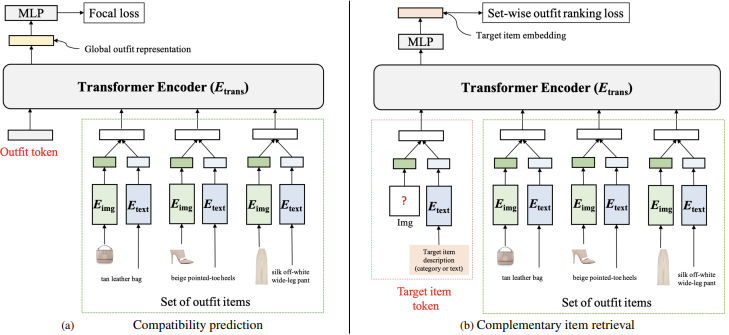
\includegraphics[scale = 0.8]{pictures/OutfitTransfromer intro.png}
	
				Предложенную модель обучают сначала для оценки совместимости образа, а затем заменяют последние линейные слои и дообучают получать представление образа для подбора подходящих элементов на основании полученного представления и текстового описания нового элемента. Из этого можно заключить, что учет внутренней структуры оказывается полезным и для оценки образа целиком, и для восстановления отдельных его частей, причем для разных задач возможно использовать одни и те же латентные представления элементов. \\
				
				Идею с общими внутренними представлениями для разных задач развивают авторы \cite{https://doi.org/10.48550/arXiv.2303.02483}. В статье рассматривается вопрос обучения мультимодального трансформера одновременно на несколько задач связанных с образами. 
				
				\begin{wrapfigure}{l}{0.52\textwidth}
					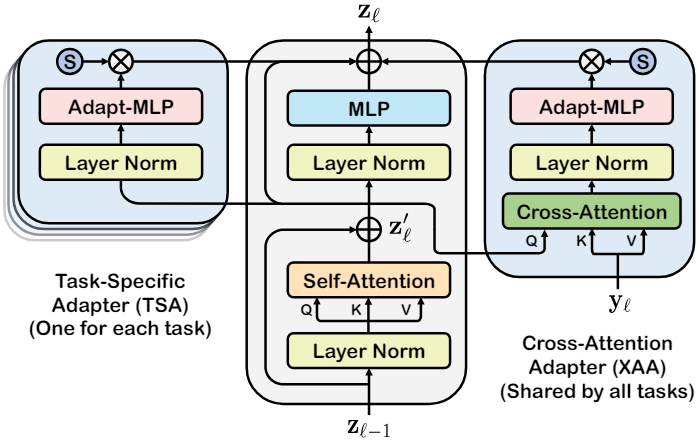
\includegraphics[scale = 1.0]{pictures/FAME-ViL_acrhitecture.png}
				\end{wrapfigure}
				
				Основой архитектуры предложенной модели выступает предтренированный CLIP \cite{https://doi.org/10.48550/arXiv.2103.00020}. Для того, чтобы приспособить модель к выполнению различных задач рекомендации, распознавания и оценки образов авторы предлагают 2 вида адаптеров: TSA -- Task-Specific Adapter для обучения специфическим для каждой задачи особенностям и XAA -- Cross-Attention Adapter для обеспечения возможности взаимодействиями между различными модальностями, общий для всех задач. Для TSA предлагается ввести дополнительные линейные слои (AdaptMLP) после каждого self-attention блока параллельно с основными:
				$$z_l^{tsa}=s \cdot AdaptMLP(LN(z'_l))$$
				где $s$ -- Обучаемый множитель.\\
				В XAA используется дополнительный Multi-Head Cross Attention (MHXA) с группой линейных слоев после него:
				$$z_l^{xaa} = s\cdot AdaptMLP(LN(MHXA(z_l',y_l)))$$
				где $y_l$ выход self-attention слоя части сети для другой модальности.\\
				Далее полученные $z_l^{tsa}$ и $z_l^{xaa}$ аггрегируются с обычным выходом следующим образом:
				$$z_l = MLP(LN(z_l')) + z_l'+z_l^{tsa}+\epsilon\cdot z_l^{xaa},~\epsilon\in\{0,1\}$$
				$\epsilon$ -- барьерный множитель включающий или выключающий определенный адаптер для определенной задачи. 
				
				Рассматриваемая архитектура обучается на разные задачи в трех режимах Contrastive, Fusion и Generative с различными используемыми адаптерами и функциями потерь. 
				
				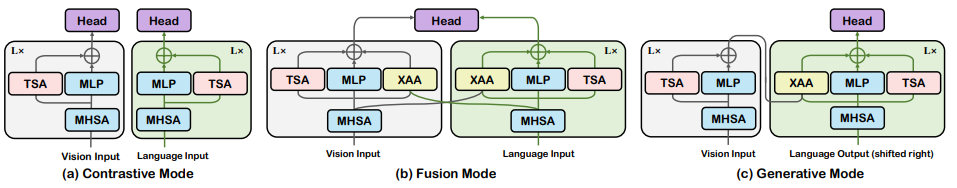
\includegraphics[scale = 0.7]{pictures/FAME-ViL_modes.png}
				
				\begin{itemize}
					\item[]\textbf{Contrastive mode:}\\
					Этот режим используется для кросс-модальных рекомендаций (XMR) --- задачи выбора наиболее подходящего элемента по текстовому описанию и выбора наиболее подходящего описания элемента на изображении среди данных. Все XAA блоки отключены. Обучение производится на выборках элементов $\mathcal{X} \supseteq (\textbf{I}, \textbf{T}) = \{(I_1, T_1), \dots, (I_B, T_B)\}$, сначала части сети для соответствующей модальности по отдельности применяются к элементам каждой пары, формируя 2 итоговых унимодальных представления, а потом с помощью контрастной функции потерь \cite{https://doi.org/10.48550/arXiv.2004.11362} производится максимизация схожести получившихся унимодальных представлений.
					$$\mathcal{L}_{XMR} = \frac{1}{2} [\mathcal{L}_{InfoNCE}(\mathbf{T}, \mathbf{I}) + \mathcal{L}_{InfoNCE}(\mathbf{I}, \mathbf{T})]$$
					$$\mathcal{L}_{InfoNCE} = -\frac{1}{B}\sum\limits_{i=1}^{B}\log\frac{\exp(s(X_i, Y_i)/\tau)}{\sum_{j=1}^B\exp(s(X_i, Y_j)/\tau)}$$
					где $\tau$ -- обучаемая температура. $s$ -- симметричная функция схожести $s(I_i, T_j) = f_\theta^{[c]}(I_i)^T\cdot f_\theta^{[c]}(T_j)$, где $f_\theta^{[c]}$ -- собственно нейросеть.
					\item[]\textbf{Fusion mode:}\\
					Используется для субкатегориального распознавания (SCR)и направляемых текстом рекомендаций (TGIR). И XAA, и TSA блоки включены. \\
					Задача SCR -- предсказание подкатегории для данного товара, основываясь на тексте и картинке. Исходя из специфики задачи, к выходу сети дополнительно добавляется классификатор, cross-entropy-loss которого и минимизируется:
					$$\mathcal{L}_{SCR} = -\mathbb{E}_{(I,T)\sim D}\log P\left(f_\theta^{[f]}(I, T)\right)$$
					Для TGIR --нахождения элементов похожих по изображению на данный и соответствующих текстовому описанию -- подход немного другой, поскольку необходимо получить представления отдельно для исходной картинки с текстовым описанием и целевой картинки, поэтому для $(\mathbf{I^r}, \mathbf{T})$ соответственно исходных картинок и текстовых запросов сеть запускается в $fusion$ режиме, а для целевых изображений $I^t$ в $contrastive$ режиме. Далее считается контрастная функция потерь вида
					$$\mathcal{L}_{TGIR} = \mathcal{L}_{InfoNCE}((I^r,T), I^t)$$
					
					\item[]\textbf{Generative mode:}\\
					Используется, например, для генерации описания к изображениям элементов. TSA блоки включены в обеих модальностях, XAA -- только image-to-text. Причем часть обрабатывающая входное изображение используется как энкодер, а вторая -- как декодер в авторегрессионном режиме.
				\end{itemize}
			
		\section{Решение задачи дополнения образа}
				Отличительной особенностью рассмотренных выше подходов является, попытка в том или ином виде моделировать взаимодействие в полном графе из частей внутренней структуры образов (элементов или признаков). Для моделирования взаимодействия между составными частями объекта или образа, нужно, для начала, получить некоторое их векторное представление. 
				
				В работе не будем сравнивать между собой способы векторизовать текстовые и графические представления и заранее их зафиксируем. Более того, сконцентрируемся на представлении образа как множества элементов без внутренней структуры и оставим вопрос разбиения объектов на признаки и рассмотрения их взаимодействия за рамками данной работы.
								
				Для получения представлений текстового и графического описания каждого элемента будем использовать предобученную модель <<Outfit Transformer>>\cite{https://doi.org/10.48550/arXiv.2204.04812}. Под множеством объектов $\mathcal{X}$ далее будем подразумевать множество их векторных представлений $\mathcal{X}\subset \mathbb{R}^d$
				
				Будем рассматривать задачу дополнения образа. Для ее решения, как было сказано, необходимо знать функцию совместимости. Оставим восстановление этой функции за рамками текущей работы и снова будем пользоваться ранее предложенным решением -- предобученной моделью из \cite{https://doi.org/10.48550/arXiv.2204.04812}, для действия этой модели на образ будем использовать обозначение введенное выше для функции оценки --- $\mathcal{S}(\cdot)$. 
				$\mathcal{S}(\cdot)$ --- ограниченная непрерывно дифференцируемая функция своих аргументов, причем норма ее градиента также ограничена. 
				
				Далее нас будет интересовать исключительно случай пустого описания недостающих элементов. Учитывая постановку определенную ранее и все названные допущения, получаем задачу следующего вида:
				\begin{itemize}
					\item[] \textbf{Дано:}\\
					$O_n\in\mathcal{O}, ~|O| = n$ --- исходный образ \\
					$k \in \mathbb{N}, ~k$ --- количество недостающих элементов\\					
					\item[] \textbf{Задача:}
					$$\{\hat{X_i}\}_{i=1}^k= \argmax_{\{X_i\}_{i=1}^k\subset\mathcal{X}} \mathcal{S}\left(O_n\cup\{X_i\}_{i=1}^k\right)$$
				\end{itemize}
				Для $k > 1$ и большого количества доступных элементов решение задачи полным перебором  становится вычислительно невозможным (сложность алгоритма полного перебора $|\mathcal{X}|^k$), поэтому необходимо рассмотреть возможные способы приближенного решения. 
				
			\subsection{Дискретный подход}\label{discrete}
			Заметим, что математически задача выбора $k$ наиболее подходящих к образу элементов может быть переформулирована как задача поиска наилучшего пути длины $k$ в полном графе, множество вершин которого есть 
			$$\mathcal{X}\setminus O_n \cup \{X_{init}\},$$ где $X_{init}$ -- дополнительная начальная вершина. Для некоторого пути $X_{init}, X_1\dots X_j$ можно рассчитать его <<\textit{оценку}>> как оценку образа $O_n\cup\{X_1\dots X_j\}$ тогда понятно, что поиск пути с максимальной оценкой эквивалентен решению поставленной выше задачи дополнения образа. Такой подход требует подсчета оценки текущего пути на каждом шаге, а значит чтобы улучшить асимптотику и получить практически вычислимый алгоритм, необходимо использовать приближенное решение задачи поиска в графе.
			
			В качестве бейзлайна будем рассматривать два следующих жадных алгоритма:
			\begin{enumerate}
				\item <<Одношаговый>> $|\mathcal{X}|$ вызовов функции оценки
				\begin{itemize}
					\item Подсчет $\mathcal{S}(O_n \cup X)$ для всех элементов $X\in \mathcal{X}$
					\item Выбор элементов $X_i,~i=\overline{1,k}$ соответствующих k максимальным значениям $\mathcal{S}(O_n \cup X)$
				\end{itemize}
				\item <<Многошаговый>> $k\cdot|\mathcal{X}|$ вызовов функции оценки
				\begin{itemize}
					\item Подсчет $\mathcal{S}(O_n \cup X)$ для всех элементов $X\in \mathcal{X}$
					\item Выбор элемента $X_1$ соответствующего максимальному значению $\mathcal{S}(O_n \cup X)$
					\item Подсчет $\mathcal{S}(O_n \cup X_0\cup X)$ для всех элементов $X\in \mathcal{X}$
					\item Продолжение последовательных итерации до $X_k$
				\end{itemize}
			\end{enumerate}
			
			Возможно обобщить жадные алгоритмы и применить широко используемый, например в языковых генеративных моделях, алгоритм beam-search, однако он либо вырождается в многошаговый алгоритм выше, либо требует еще больше чем $k\cdot|\mathcal{X}|$ вызовов функции оценки для каждого образа, что ставит под вопрос практическую применимость.
			
			\subsection{Непрерывный подход}\label{continuous}
			Как альтернативу приближенному перебору можно рассмотреть решение релаксированной задачи во всем пространстве $\mathbb{R}^d$
			$$\{\tilde{X_i}\}_{i=1}^k= \argmax_{\{X_i\}_{i=1}^k\subset\mathbb{R}^d} \mathcal{S}\left(O_n\cup\{X_i\}_{i=1}^k\right)$$
			Поскольку мы пользуемся предобученной моделью для подсчета функции оценки, нам доступны не только ее значения для любого образа, но и градиент в любой точке. Значит, такой постановке $\{\tilde{X_i}\}$ могут быть найдены например одной из вариаций градиентного спуска.
			Далее 
			$$\hat{X_i} =  \argmin_{X\in\mathcal{X}} \rho(\tilde{X_i}, X),$$
			где $\rho$ -- некоторая метрика, например $L_p$. 
			$\mathcal{S}$ -- непрерывно дифференцируемая функция с ограниченным по норме градиентом, а значит липшицева с некоторой константой $M$, в таком случае:
			$$\sum_{i=1}^k\rho(\hat{X_i}, \tilde{X_i}) < \varepsilon\longrightarrow \biggr{|}\mathcal{S}\left(O_n\cup\{\tilde{X_i}\}_{i=1}^k\right) - \mathcal{S}\left(O_n\cup\{\hat{X_i}\}_{i=1}^k\right)\biggr{|} < M\cdot\varepsilon$$
			Что позволяет надеяться на хорошие результаты при достаточном количестве данных.
			
			К минусам подхода можно отнести сохраняющуюся необходимость многократного вызова функции $\mathcal{S}$ и ее градиента для решения оптимизационной задачи в $\mathbb{R}^d$, однако количество итераций градиентного спуска в этом случае по крайней мере не зависит от размеров используемого датасета.\\
			Кроме того, 
			$$\sum_{i=1}^k\rho(\hat{X_i}, \tilde{X_i}) < \varepsilon$$
			довольно сильное условие на непрерывное решение и для того, чтобы оно выполнялось, необходимо по крайней мере
			$$\exists \{\hat{X_i}\}_{i=1}^k\subset\mathcal{X}:~ \mathcal{S}\left(O_n\cup\{\hat{X_i}\}_{i=1}^k\right) \geqslant \max_{\{X_i\}_{i=1}^k\subset\mathbb{R}^d} \mathcal{S}\left(O_n\cup\{X_i\}_{i=1}^k\right) - M\varepsilon$$
			$$\Updownarrow$$
			$$\max_{\{X_i\}_{i=1}^k\subset\mathcal{X}} \mathcal{S}\left(O_n\cup\{X_i\}_{i=1}^k\right) \geqslant \max_{\{X_i\}_{i=1}^k\subset\mathbb{R}^d} \mathcal{S}\left(O_n\cup\{X_i\}_{i=1}^k\right) - M\varepsilon$$
			
			Таким образом, релаксация задачи до непрерывной и решение ее градиентным спуском может иметь смысл только в случае наличия очень богатой коллекции, для которой с нужной точностью выполнено условие выше, и возможности достаточно быстро решить задачу с помощью градиентного спуска. Теоретическая оценка того, с какой точностью выполнены эти условия затруднительна, поэтому возможность применимости будем рассматривать в вычислительном эксперименте на примере конкретного датасета.
						
			\subsection{Генерация взаимосвязанных скрытых представлений}\label{generation}
			Чтобы гарантировать возможность быстрого применения алгоритма на практике, необходимо рассмотреть сведение количества применений функции оценки или другой функции аппроксимированной нейронной сетью к минимуму. Для этого в предложенном ниже методе полностью откажемся от вызова функции оценки на этапе применения и переформулируем задачу как поиск аппроксимации функции 
			$$\mathcal{F}^{(k)}: \mathcal{O}\longrightarrow \mathcal{X}^k, ~~~O_n\in \mathcal{O},~ \mathcal{F}^{(k)}(O_n) = \argmax_{\{X_i\}_{i=1}^k\subset\mathcal{X}} \mathcal{S}\left(O_n\cup\{X_i\}_{i=1}^k\right)$$
			
			Композицией функций 
			$$F^{(k)}_\mathbf{\theta}: \mathcal{O}\longrightarrow \mathbb{R}^d, ~F^{(k)}_\mathbf{\theta}(O_n) = \{X_i\}_{i=1}^k$$
			
			 $$\text{и }\rho_\mathcal{X}: \mathbb{R}^d\longrightarrow \mathcal{X}, ~ \rho_\mathcal{X}(X_i) = \argmax_{\hat{X_i}\in\mathcal{X}}\rho(X_i, \hat{X_i})$$
			$\rho(\cdot, \cdot)$ -- некоторая мера близости между аргументами, позже в эксперименте попробуем выбрать наиболее подходящую из некоторых популярных вариантов.
			 
			Таким образом мы свели исходную задачу к задаче генерации скрытых представлений недостающих элементов $\{\hat{X_i}\}\subset \mathbb{R}^d$, наиболее близких в смысле функции $\rho$ к точным решениям задачи
			$$\{\hat{X_i}\}_{i=1}^k= \argmax_{\{X_i\}_{i=1}^k\subset\mathcal{X}} \mathcal{S}\left(O_n\cup\{X_i\}_{i=1}^k\right)$$
			с помощью функции  $F^{(k)}_\mathbf{\theta}$ с вектором параметров $\mathbf{\theta}$. 
			
			Эту функцию предлагается приближать нейронной сетью. Как и 
			Для обучения сети требуется набор точных решений задачи, тогда как в используемых на практике датасетах только очень малая доля всех образов имеет оценку близкую к максимально возможной, а значит необходимо предложить способ получения точного решения или его приближения за конечное время. Лучшим из рассмотренных методов, очень близким к полному перебору, является многошаговый жадный подход описанный в \ref{discrete}. 
			
			Таким образом, предлагается двухэтапный процесс построения модели генерации представлений для дополнения образа:
			\begin{enumerate}
				\item Для подмножества множества образов 
				$$\mathcal{O}_n = \{O^i\}_{i=1}^n \subset\mathcal{O}$$
				 с помощью многошагового жадного метода сгенерировать приближенные решения задачи дополнения образа $$\mathcal{X}_n =\{\{\tilde{X_j^i}\}_{j=1}^k\}_{i=1}^n\subset\mathcal{X}^k$$
				  
				\item\label{step2} Обучить нейронную сеть для функции $F^{k}_\mathbf{\theta}$ используя $\mathcal{O}_n$ и $\mathcal{X}_n$ в качестве обучающих данных, т.е. решить оптимизационную задачу следующего вида:
				$$\hat{\theta} = \argmin_\theta \frac{1}{n}\sum_{i=1}^n\sum_{j=1}^k\rho\left(\tilde{X_j^i}, \left[F^{(k)}_{\theta}(O^i)\right]_j\right)$$
				Далее, как сказано выше, в качестве ответа выбираем
				$$X_j^i = \rho_\mathcal{X}\left(\left[F^{(k)}_{\hat{\theta}}(O^i)\right]_j\right) = \argmax_{\hat{X_i}\in\mathcal{X}}\rho\left(\left[F^{(k)}_{\hat{\theta}}(O^i)\right]_j, \hat{X_i}\right)$$
			\end{enumerate}
		
		
		Задача по постановке симметрична к перестановкам элементов, поэтому разумно потребовать от всех операций в архитектуре сети эквивариантности \cite{cohen2016group} к перестановкам. Кроме того, эмпирически понятно, что элементы в образе сложным образом зависимы друг от друга.
		Ничего больше про внутреннюю структуру данных неизвестно, поэтому в таком случае естественным будет рассмотреть применение графовых нейросетей для аппроксимации функции $F_k^\mathbf{\theta}$, поскольку они эквивариантны к перестановкам по построению и хорошо показывают себя в задачах требующих моделирования сложных взаимодействий между объектами схожей природы.
		
		Тогда, используя message passing GNN из \ref{GNN}, приняв $\theta = \{\alpha_t, \beta_t\}_{t=1}^{T}$, где $T$ количество слоев в сети, и используя функцию суммы в качестве аггрегационной для <<сообщений>>, запишем функцию $F^{k}_{\theta}$ следующим образом:
		$$F^{(k)}_{\theta}(O^i) = F^{(k)}_{\theta}(O^i_1,\dots O^i_m) = f_\theta^{(T)}\left(\dots \left(f_\theta^{(1)}(O^i_1,\dots O^i_m, x_1, \dots x_k)\right)\dots\right),$$
		где $x_1,\dots x_k$ --- векторы признаков в случайно инициализированных вершин графа, соответствующих $k$ элементам дополнения, а $f_\theta^{(t)}$ есть применение $t$-го слоя к скрытым представлениям предыдущего, т.е.:
		$$\left[f^{(t)}_\theta \left(h_1^{(t)}\dots h_{m+k}^{(t)}\right)\right]_j\! = U_{\alpha_t}^t\left(h^{(t)}_j, \sum_{i=1}^{m+k} M_{\beta_t}^{(t)}\left(h^{(t)}_j, h^{(t)}_i\right)   \right),$$
		здесь $U_{\alpha_t}^t, M_{\beta_t}^{(t)}$ обучаемые преобразования на слое $t$ с параметрами $\alpha_t$ и $\beta_t$ соответственно.
		
		Подставляя это выражение в оптимизационную задачу на шаге \ref{step2}, получаем наконец задачу минимизации для обучения нейронной сети генерации представлений ближайших к наилучшему приближению точного решения исходной задачи.
		
		Используя сеть такого вида можно генерировать скрытые представления одновременно для $k$ элементов, в отличие от всех ранее представленных подходов, осуществляющих последовательное добавление в образ по одному элементу. Это повышает эффективность в $k$ раз, а также позволяет в процессе генерации моделировать взаимодействие в том числе между новыми элементами.
		
		
		\section{Вычислительный эксперимент}
			\subsection{Условия эксперимента}
					Для эксперимента мы используем датасет Polyvore \cite{DBLP:journals/corr/HanWJD17} объемом  $\sim60000$ элементов. Доступным для алгоритмов сделаем все множество элементов датасета, а для сравнения качества выберем 1000 случайных неполных образов. Кроме того зафиксируем количество элементов дополнения $k=2$. 										
					
					Понятно, что тем лучше метод, чем выше в среднем оценка образов, полученных с помощью него. Однако, оценка исключительно по среднему не вполне репрезентативна, поэтому для сравнения рассмотренных алгоритмов будем считать оценку каждого из 1000 получившихся образов, строить гистограмму получившегося распределения оценок и считать его выборочную медиану
					
					Из рассмотренных алгоритмов наилучшим приближением точного решения задачи являются алгоритмы жадного перебора, хоть время необходимое для получения с помощью них результата и слишком велико для применения на практике. Тем не менее, будем рассматривать решения полученные жадным образом как наилучший достижимый за ограниченное время бейзлайн и оценивать насколько более быстрые алгоритмы смогут к нему приблизиться. Кроме того, для сравнения будем наносить на каждый график гистограмму распределения оценок исходных образов из датасета. 
					
			\subsection{Жадные алгоримты}
				Будем тестировать 2 алгоритма описанных в \ref{discrete} соответственно <<одношаговый>> и <<многошаговый>>.
				\begin{center}
					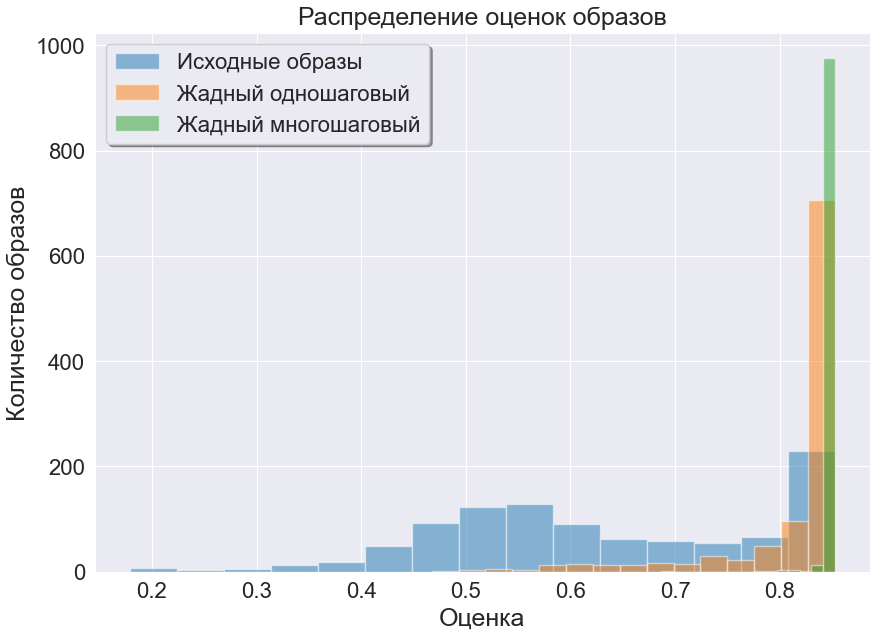
\includegraphics[scale = 0.6]{../figures/greedy_at_least_5_subset1000.png}
				\end{center}
				Как и ожидалось результат близок к идеальному -- оценки почти всех получившихся образов близки к 1, однако вычисление в цикле длины пропорциональной размеру датасета делает алгоритм практически неприменимым. 
				
			\subsection{Непрерывный подход}\label{continuous test}
			Исследуем качество и применимость алгоритма из \ref{continuous} для нескольких популярных функций близости -- рассмотрим в качестве $\rho$ метрики $L_1$, $L_2$ и $L_{10}$ и косинусное расстояние. Теоретический анализ в высокоразмерном пространстве неизвестной структуры затруднен, но исходя из сравнительного анализа в \cite{shirkhorshidi2015comparison} стоит ожидать, что лучий результат будет показывать косинусное расстояние, однако утверждать без эксперимента невозможно, поэтому проверим, что будет подходить лучше на практике. Кроме того, сложно оценить насколько датасет удовлетворяет условиям описанным в \ref{continuous} и прогнозировать хороший результат.
			
			\begin{center}
				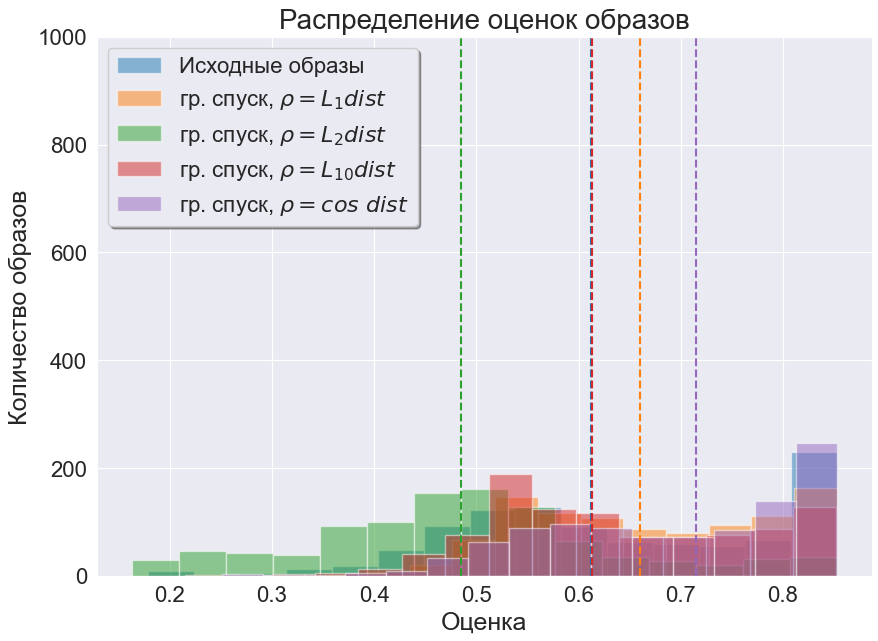
\includegraphics[scale = 0.6]{../figures/backprop_at_least_5_subset1000.png}
			\end{center}
			По итогам тестирования алгоритма решения задачи с помощью релаксации до непрерывной можно сказать, что выбор нормы сильно влияет на результат -- лучше всего, как и предполагалось, себя показывает косинусное расстояние. Оценки полученных дополнений даже в лучшем случае лишь немногим превосходят исходные и серьезно уступают результатам жадных алгоритмов, а скорость работы крайне низка из-за необходимости для каждого образа проводить $\sim$1000 итераций градиентного спуска (до достижения сходимости), хоть и не зависит от размера выборки.
			
			\subsection{Генерация скрытых представлений}
				Наконец перейдем к основному алгоритму рассматриваемому в работе, описанному в \ref{generation}. Аналогично решению релаксированной задачи, будем рассматривать 4 различных функции $\rho$: метрики $L_1, L_2, L_{10}$ и косинусное расстояние. Будем рассматривать довольно простую архитектуру сети: в качестве $M^{(t)}_{\beta_t}$ возьмем композицию применения двух разных линейных слоев соответственно к двум аргументам и сумму двух результатов, в качестве $U^{(t)}_{\alpha_t},$ композицию линейного слоя и функции активации ReLU, примем $T=4$. Будем обучать сеть на дополнения полученные для использованных выше 1000 образов с помощью многошагового жадного алгоритма из \ref{discrete}. Тестировать будем на тренировочной выборке и на отложенной из других 1000 образов случайно, выбранных из датасета.
				
				Оценки дополненных образов соответственно из тренировочной и тестовой выборок для различных функций близости следующие:
				
				\begin{figure}[h!]
					\begin{subfigure}[b]{0.5\linewidth}
						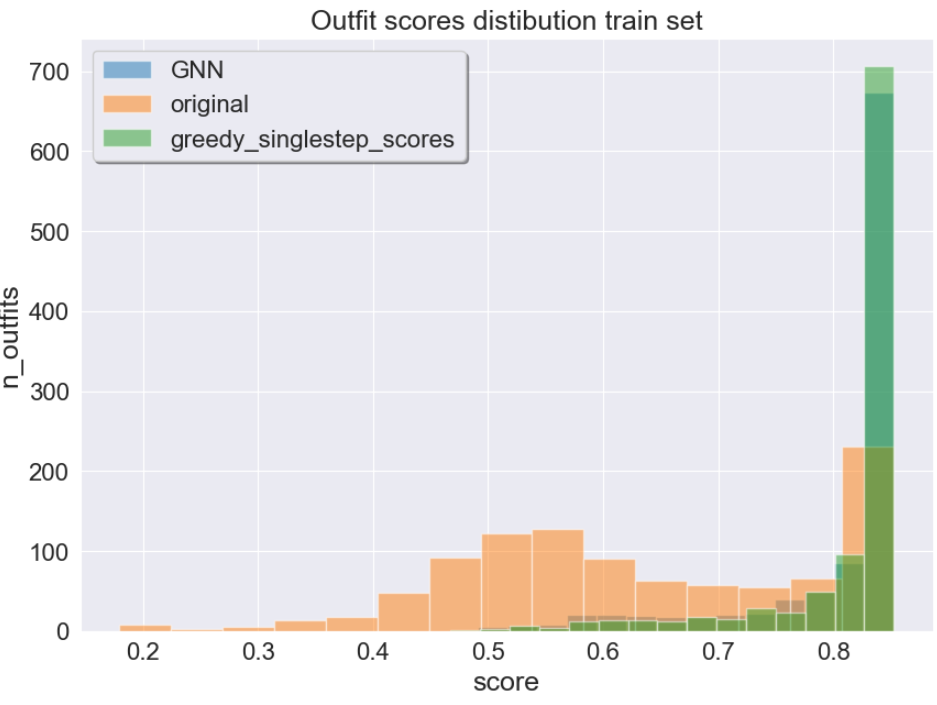
\includegraphics[scale = 0.5]{../figures/GNN_at_least_5_subset1000_train.png}
					\end{subfigure}
					\hfill
					\begin{subfigure}[b]{0.5\linewidth}
						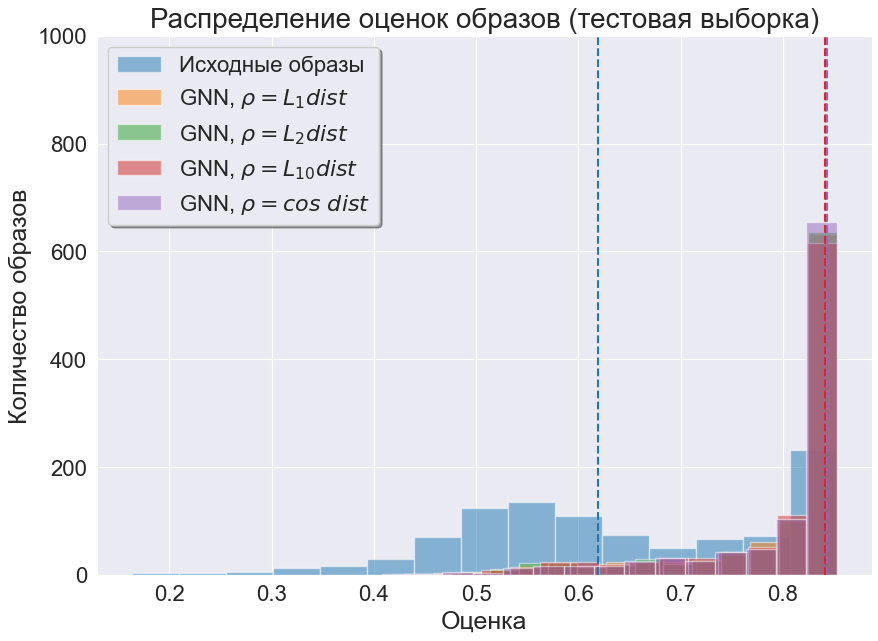
\includegraphics[scale = 0.5]{../figures/GNN_at_least_5_subset1000_test.png}
					\end{subfigure}
				\end{figure}
			
				Интересно, что, в отличие от эксперимента с релаксированной задачей \ref{continuous test}, выбор функции близости не оказывает такого серьезного влияние на распределение итоговых оценок, несмотря на большую размерность пространства элементов, хотя результат для косинусного расстояния все равно немного лучше. Это можно объяснить тем, что хорошо обученная сеть генерирует достаточно близкие к целевым ответы, и <<ближайшими>> в датасете в смысле любой из этих функций оказываются элементы, оценка образа с которыми близка к оценке образа с целевыми в силу липшицевости, о чем подробней написано в \ref{continuous}. 
				
				Теперь приведем сравнение с жадным алгоритмом. Понятно, что достичь качества многошагового невозможно, поскольку мы обучаем сеть на его ответы. В сравнении с одношаговым же получаем следующее:
				
				\begin{center}
					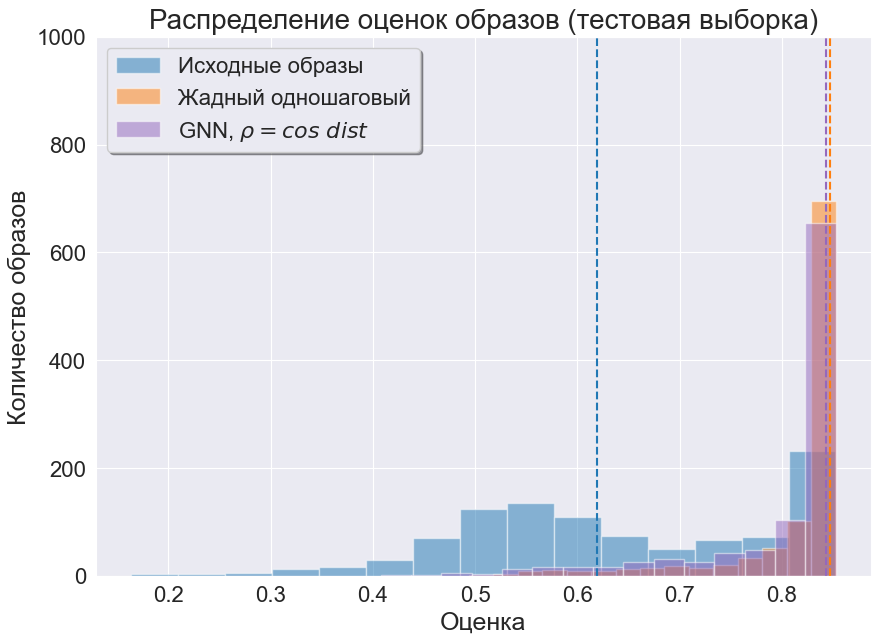
\includegraphics[scale = 0.6]{../figures/GNN_at_least_5_subset1000_test_comparison.png}
				\end{center}
									
				Таким образом, качество решения задачи дополнения с помощью прямой генерации скрытых представлений лишь немногим уступает полученному одношаговым алгоритмом, но осуществляется быстрее на 2 порядка даже при сравнительно небольшом датасете, использованном в эксперименте. Это дает возможность применять его на практике, не жертвуя качеством.
				
				\subsection{Сравненительная таблица}
				\begin{center}
%					\begin{table}[h]
						\begin{tabular}{|c|cccc|}
							\hline
							\multirow{2}{*}{$\rho$} & \multicolumn{4}{c|}{Выборочная медиана оценок образов}                                                                       \\ \cline{2-5} 
							& \multicolumn{1}{c|}{ж. однош.}            & \multicolumn{1}{c|}{ж. многош.}           & \multicolumn{1}{c|}{гр. спуск} & GNN \\ \hline
							$L_1$                   & \multicolumn{1}{c|}{\multirow{4}{*}{0.8511}} & \multicolumn{1}{c|}{\multirow{4}{*}{0.8467}} & \multicolumn{1}{c|}{0.6602}         & 0.8417    \\ \cline{1-1} \cline{4-5} 
							$L_2$                   & \multicolumn{1}{c|}{}                     & \multicolumn{1}{c|}{}                     & \multicolumn{1}{c|}{0.4850}         & 0.8417  \\ \cline{1-1} \cline{4-5} 
							$L_{10}$                & \multicolumn{1}{c|}{}                     & \multicolumn{1}{c|}{}                     & \multicolumn{1}{c|}{0.6132}         &  0.8415  \\ \cline{1-1}\cline{4-5} 
							$cos~dist$              & \multicolumn{1}{c|}{}                     & \multicolumn{1}{c|}{}                     & \multicolumn{1}{c|}{0.7142}         &  0.8428  \\ \hline
							Задержка, с             & \multicolumn{1}{c|}{4}                     & \multicolumn{1}{c|}{8}                     & \multicolumn{1}{c|}{5}          &   0.03  \\ \hline
						\end{tabular}
%					\end{table}
				\end{center}
			\newpage
			
			
			\section{Заключение}
				В работе подробно рассмотрена задача дополнения образа и существующие подходы к ее решению, а также к решению сопутствующих задач. Обоснована невозможность получить точное решение, а также неприменимость на практике его аппроксимаций с помощью перебора. Рассмотрено 2 возможных альтернативных метода решения:  решение релаксированной задачи в непрерывном пространстве 
				\ref{continuous} и прямая генерация скрытых представлений решения \ref{generation}. Первый, несмотря на теоретическое обоснование, вероятно, из-за не выполнения предположения описанного в \ref{continuous}, проверить которое довольно трудно, на эксперименте 		доказал свою несостоятельность для выбранных данных --- время его работы слишком велико, а итоговое качество довольно низко. Для второго получено теоретическое обоснование без дополнительных предположений, в том числе обосновано применение для приближения параметрической функции в нем графовой нейронной сети. Кроме того, предложен и обоснован способ пополнения обучающей выборки для модели генерации, в условиях недостатка в рассматриваемых данных образов с высокой оценкой. 
				На основании эксперимента, можно утверждать, что метод генерации представлений может быть успешно применен для прикладных задач, так как качество образов, полученных с помощью близко к наилучшему достижимому за ограниченное время (с помощью жадных алгоритмов), а время работы для одного образа $<50$мс на современном ноутбуке.
				
			
	\bibliographystyle{plain}
	\bibliography{references}
			
	 
\end{document}